\chapter{la Tour de Hanoi, historique et présentation du problème}

\section{Introduction Historique}
La Tour de Hanoi est inspirée à Lucas par l’un de ses amis, le professeur Claus de Siam qui raconte une histoire ayant lieu au coeur du temple Kashi Vishwanath :
Trois aiguilles de diamant, plantées dans une dalle d’airain. […] Sur une de ces aiguilles, Dieu enfila au commencement des siècles, 64 disques d’or pur, le plus large reposant sur l’airain, et les autres, de plus en plus étroits, superposés jusqu’au sommet.

C’est la tour sacrée du Brahmâ. Nuit et jour, les prêtres se succèdent sur les marches de l’autel, occupés à transporter la tour de la première aiguille sur la troisième, sans s’écarter des règles fixes que nous venons d’indiquer, et qui ont été imposées par Brahma. Quand tout sera fini, la tour et les brahmes tomberont, et ce sera la fin des mondes !

Edouard Lucas, Récréations mathématiques, tome 3, (1892), réédité par la Librairie Albert Blanchard, (1979), p. 58
\subsection{fait amusant}
Comme indiqué ci-dessous, un jeu à 64 disques requiert un minimum de 264-1 déplacements (soit 18 446 744 073 709 551 615 déplacements). En admettant qu'il faille 1 seconde pour déplacer un disque, ce qui fait 86 400 déplacements par jour, la fin du jeu aurait lieu au bout d'environ 213 000 milliards de jours, ce qui équivaut à peu près à 584,5 milliards d'années, soit 43 fois l'âge estimé de l'univers (13,7 milliards d'années selon certaines sources)

\section{Présentation du problème}
Les tours de Hanoï (originellement, la tour d'Hanoïa) sont un jeu de réflexion imaginé par le mathématicien français Édouard Lucas, et consistant à déplacer des disques de diamètres différents d'une tour de « départ » à une tour d'« arrivée » en passant par une tour « intermédiaire », et ceci en un minimum de coups, tout en respectant les règles suivantes :

->on ne peut déplacer plus d'un disque à la fois.
->on ne peut placer un disque que sur un autre disque plus grand que lui ou sur un emplacement vide.

\begin{figure}[H]
    \centering
        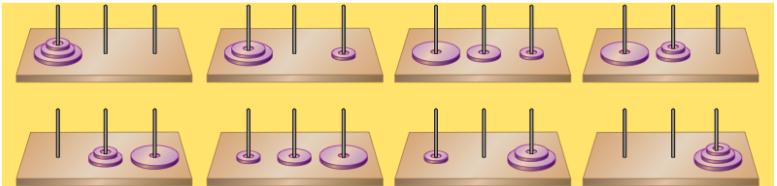
\includegraphics[scale=0.5]{./ressources/Présentation_du_problème.png}
        \caption{Exemple d'une solution dans le cas de trois disques}
    \label{fig:representationProbleme}
\end{figure}

\subsection{Polémique}
Il existe toujours cette confusion dans certains articles scientifiques qui mentionnent que le problème de la tour de Hanoi est NP alors que ce n'est pas le cas.

Dans ce problème les étapes correctes peuvent être déterminées dès le départ sans avoir besoin d'une recherche d'essais-erreurs pour prendre la bonne décision. Par conséquent, ce problème n'est pas un problème de décision, auquel des classes telles que NP s'appliquent.

C'est plus un problème de fonction. La complexité temporelle est en effet déterminée par le nombre d'étapes à sortir, qui est de $2^{n-1}$, c'est-à-dire $O(2^n).$
La classe correspondante serait donc FEXPTIME-Complete, le préfixe F signifiant Function, et Complete signifiant que cela ne peut se faire en un temps inférieur à exponentiel (comme P). Elle est analogue à la classe EXPTIME-Complete pour les problèmes de décision, c'est-à-dire $O(2^{polynomial(n)})$.

Il faut savoir que la classe EXPTIME En théorie de la complexité, est la classe de complexité qui est l'ensemble des problèmes de décision décidés par une machine de Turing déterministe en temps exponentiel.  Mais il existe des classes plus grosses comme EXPSPACE et NEXPTIME (respectivement les problèmes pouvant être résolus en espace exponentiel, et en temps exponentiel sur machine non déterministe).
L'illustration ci-dessous montre le diagramme d'inclusions des classes de complexité classiques :
\begin{figure}[H]
    \centering
        \includegraphics[scale=0.5]{./ressources/Les_classes_de_complexité.png}
        \caption{Diagramme d'inclusions des classes de complexité classiques.}
    \label{fig:classeComplexite}
\end{figure}

\subsection{Définition formelle du problème}
Il est facile de démontrer par récurrence que si n est le nombre de disques, il faut 2n - 1 coups au minimum pour parvenir à ses finsc, quantité qui augmente très rapidement avec n. En effet, soient A, B et C les trois emplacements des tours ; notons $x_n$ le nombre de déplacements de disques nécessaires au déplacement d'une tour complète. Pour déplacer une tour de n disques de A vers C, on effectue ces trois étapes :

déplacer la tour des n-1 premiers disques de A vers B (étape qui nécessite $x_{n-1}$ déplacements, d’où la récurrence) ;
déplacer le plus grand disque de A vers C (un déplacement supplémentaire) ;
déplacer la tour des n-1 premiers disques de B vers C (à nouveau $x_{n-1}$ déplacements).
Le nombre de déplacements de disques vérifie donc la relation de récurrence :

\hspace*{6.4cm}                        $x_0 = 0$ \\
\hspace*{7cm}                        $x_n = 2x_{n-1}+1$ si $n >= 1$ \\
ce qui donne bien : \\
\hspace*{7cm}                        $x_n = 2^n - 1$ \\

On peut montrer que la méthode décrite ici donne la séquence optimale (celle qui nécessite le moins de coups), et que celle-ci est unique. En effet, pour déplacer la tour de n disques de A vers C, on devra forcément, à un moment ou à un autre, déplacer le plus grand disque de A vers C, et pour ce faire, on devra avoir empilé les n-1 premiers disques en B.

\section{Conclusion}
Dans ce chapitre on a parlé de l'origine du problème de la tour de hanoi et on l'a expliqué  d'une manière classique et générale. Dans ce qui suit, on présentra notre solution récursive ainsi que des exemples démonstratifs. 
